\documentclass[a4paper]{article}

\usepackage{mhchem}%化学符号的宏包
\usepackage{cite}%多个文献引用
\usepackage{graphicx}
\usepackage{array}%调节表格行高
\usepackage{multirow,makecell}%多行表格
\usepackage{tabularx}%表格固定列宽
\usepackage{subfigure}
\usepackage{titlesec}%标题格式设置
\usepackage{amsmath}
\usepackage{amssymb}
\usepackage{tabularx}
\usepackage{makecell}
\usepackage{geometry}
\usepackage{float}
\usepackage{setspace}%行距包
\usepackage{siunitx}
\usepackage{mdwlist}
\usepackage{tabu}
\usepackage{enumerate}

\geometry{top=1.54cm,bottom=2.54cm,left=2.5cm,right=2.5cm}


\begin{document}
\begin{center}
\bf\Large
EE 105 Feedback Control Systems\par
Department of Electrical and Computer Engineering\par
Tufts University Fall 2018\par
Homework \#3\par   
\end{center}
\begin{table}[H]
\begin{center}
\begin{tabular*}{\textwidth}{@{\extracolsep{\fill}}lcr}
Name: {\it Shang Wang} &Student ID: {\it 1277417} &E-mail: {\it shang.wang@tufts.edu}\\
\hline
\end{tabular*}
\end{center}
\end{table}

\section{Problem 1}
\subsection{Section A}
The transfer function of this open-loop system , while $W = 0$ is:
$$
\frac{Y(s)}{R(s)} = \frac{b}{ms+b}
$$
\subsection{Section B}
The transfer function of the close-loop system, while $W = 0$ is(using Black's formula):
$$
\frac{Y(s)}{R(s)} =\frac{\frac{B}{ms+b}}{1 + \frac{B}{ms+b}} = \frac{B}{ms+b+B}
$$
\subsection{Section C}
When $r(t) = \varepsilon(t)$($\varepsilon(t)$ is unit step function), $R(s) = 1/s$, $Y(s)$ of open loop system should be:
$$
Y(s) = \frac1s\frac{b}{ms+b} = \frac{b}{m}\frac{1}{(s+b/m)s} = \frac1s - \frac{1}{s+b/m}
$$
So $y(t)$ should be:
$$
y(t) = \mathcal{L}^{-1} (Y(s)) = \varepsilon(t)(1-e^{-\frac bmt})
$$
\subsection{Section D}
When $r(t) = \varepsilon(t)$, $R(s) = 1/s$, $Y(s)$ of close loop system should be:
$$
Y(s) = \frac1s\frac{B}{ms+b+B}= \frac{B}{m}\frac{1}{s+\frac{B+b}{m}}\frac1s = \frac{B}{B+b} \Big(\frac{1}{s}-\frac{1}{s+\frac{B+b}{m}}\Big)
$$
So $y(t)$ should be:
$$
y(t) = \mathcal{L}^{-1} (Y(s)) = \frac{B}{B+b} \varepsilon(t)(1-e^{-\frac{B+b}{m}t})
$$
\subsection{Section E}
\begin{figure}[H]
\centering
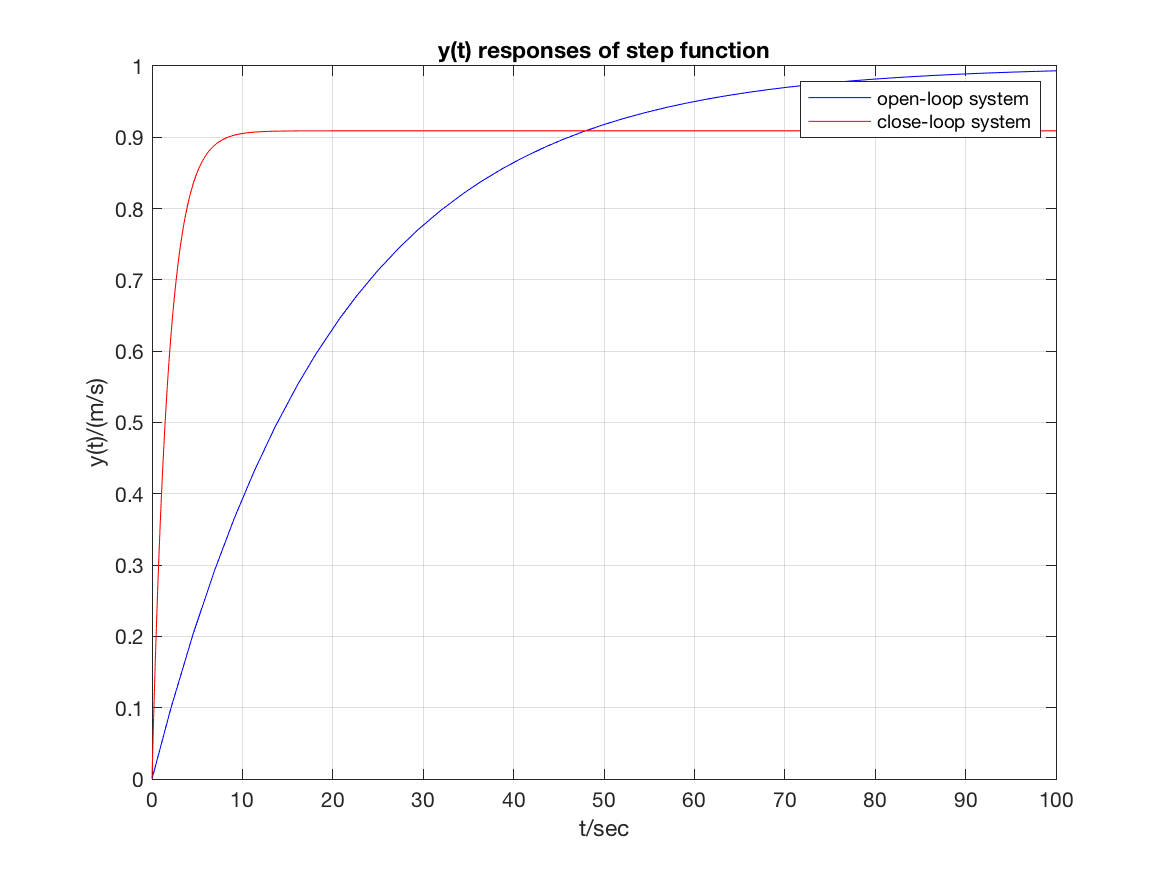
\includegraphics[width = 0.5\textwidth]{pic/e.png}

\end{figure}

\subsection{Section F}
If we let $t\rightarrow \infty$ for close-loop system, the transfer function $y(t)$ becomes:
$$
\lim_{t\rightarrow \infty}(1 - y(t)) = 1- \lim_{t\rightarrow \infty}\frac{B}{B+b} u(t)(1-e^{-\frac{B+b}{m}t}) = 1-\frac{B}{B+b} = \frac{1}{1+B/b} 
$$

\subsection{Section G}
The transfer function for the controller effort in open-loop system is:
$$
\frac{U(s)}{R(s)} = b
$$
\subsection{Section H}
The transfer function for the controller effort in close-loop system is(using Black's formula):
$$
\frac{U(s)}{R(s)} = \frac{B}{1+B/(ms+b)} = \frac{B/(ms+b)}{ms+b+B}
$$
\subsection{Section I}
When $r(t) = \varepsilon(t)$, $R(s) = 1/s$, $U(s)$ of open-loop system should be:
$$
U(s) = \frac bs
$$
So we have $u(t)$:
$$
u(t) = b\varepsilon(t)
$$

\subsection{Section J}
When $r(t) = \varepsilon(t)$, $R(s) = 1/s$, $U(s)$ of close-loop system should be:
$$
U(s) = \frac 1s\frac{B/(ms+b)}{ms+b+B} = \frac{B}{b(B+b)}\frac 1s - \frac 1b\frac{1}{s+b/m}+\frac{1}{B+b}\frac{1}{s+(B+b)/m}
$$
So we have $u(t)$:
$$
u(t) = \frac{B}{b(B+b)}\varepsilon(t)- \frac 1b\varepsilon(t)e^{-\frac bm t} + \frac{1}{B+b}\varepsilon(t)e^{-\frac{B+b}{m}t}
$$

\subsection{Section K}
\begin{figure}[H]
\centering
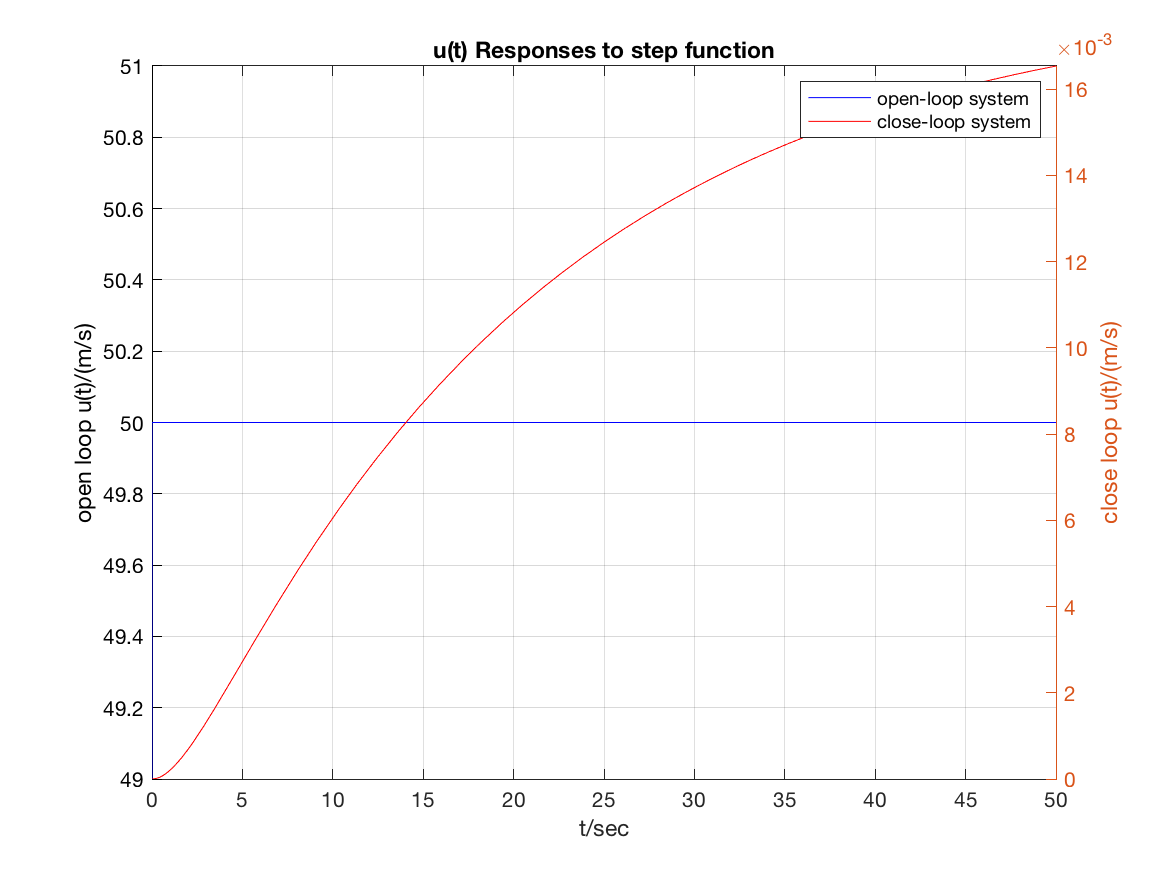
\includegraphics[width = 0.5\textwidth]{pic/k.png}
\end{figure}

\subsection{Section L}
The transfer function for the disturbance effort in open-loop system is:
$$
\frac{Y(s)}{W(s)} = \frac{1}{ms+b}
$$

\subsection{Section M}
The transfer function for the disturbance effort in close-loop system is(Using Black's formula):
$$
\frac{Y(s)}{W(s)} = \frac{1/(ms+b)}{1+B/(ms+b)} = \frac{1}{ms+B+b}
$$

\subsection{Section N}
For the open-loop system, if $W(s) = 1/s$ then:
$$
Y(s) = \frac1s\frac{1}{ms+B+b} = \frac{1}{b}\Big(\frac 1s -\frac{1}{s+b/m}\Big)
$$
So $y(t)$ is:
$$
y(t) = \frac 1b\varepsilon(t)(1-e^{-\frac bm t})
$$
For the close-loop system, we have:
$$
Y(s) = \frac 1s\frac{1}{ms+B+b} = \frac{1}{B+b} \Big(\frac 1s -\frac{1}{s+(B+b)/m}\Big)
$$
So $y(t)$ of close-loop system is:
$$
y(t) = \frac{1}{B+b}\varepsilon(t)(1-e^{-\frac {B+b}{m}t})
$$
Here is the plot:
\begin{figure}[H]
\centering
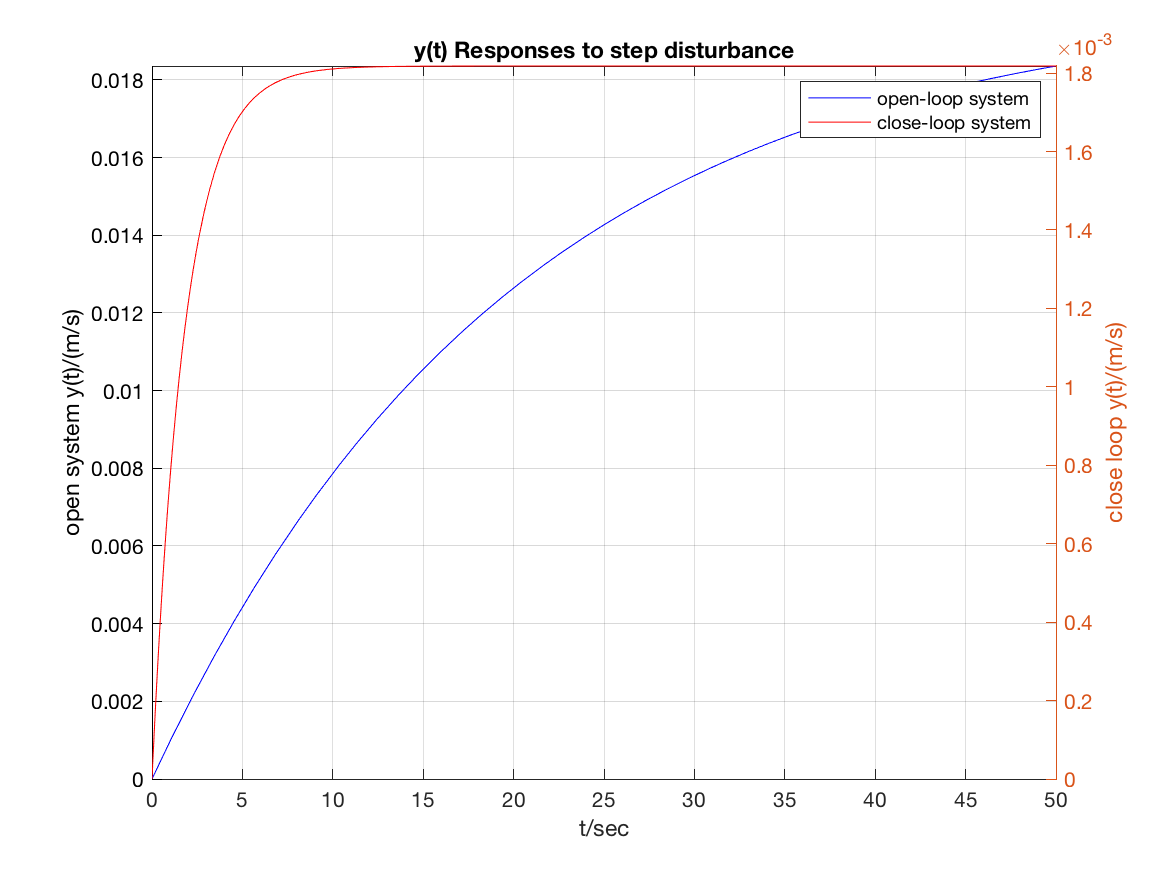
\includegraphics[width = 0.5\textwidth]{pic/n.png}
\end{figure}


















\end{document}